% Floats of Appendices C and D; see the comment in main.tex.
\begin{figure}[t]
 \centering
 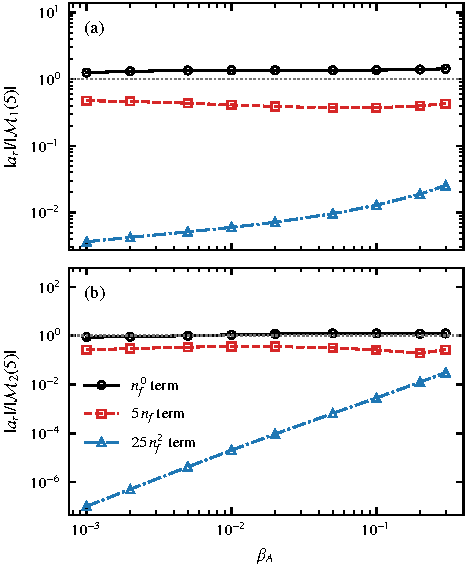
\includegraphics[width=\columnwidth]{figures/fig2_flavour.pdf}
 \caption{Magnitudes of the three terms of Eq.~\eqref{eq:nf5-sum}, divided by the magnitude of the complete coefficient, for $c=\BenchCos$, $\mA=\muR=\BenchMA\,\mathrm{GeV}$ and $\Nc=\BenchNc$. The horizontal line marks unity.}
 \label{fig:flavour-components}
\end{figure}

\begin{table}[t]
\centering
\caption{Evaluation time for the two complete Type II coefficients at the benchmark parameters, $c=\TimingCos$ and \TimingPrecision-digit working precision, for the unexpanded remainders (exact) and the series. First calls start with empty caches; repeated times are medians of \TimingRepeats{} evaluations at the same point. Starting the kernel and loading the files are excluded.}
\label{tab:timing}
\begin{ruledtabular}
\footnotesize
\setlength{\tabcolsep}{2.6pt}
\begin{tabular}{lcccccc}
& \multicolumn{3}{c}{first call [s]} & \multicolumn{3}{c}{repeated [s]} \\
$\bA$ & exact & series & ratio & exact & series & ratio \\
\hline
$1/10$ & 56.04 & 11.61 & 4.83 & 0.3422 & 0.0178 & 19.18 \\
$1/5$ & 45.68 & 11.64 & 3.92 & 0.3403 & 0.0179 & 18.99 \\
$3/10$ & 44.64 & 11.64 & 3.84 & 0.3485 & 0.0181 & 19.22 \\
\end{tabular}
\end{ruledtabular}
\end{table}

